\documentclass[12pt, a4paper]{ctexart}
\usepackage{geometry}
\geometry{left=2.5cm, right=2.5cm, top=2.5cm, bottom=2.5cm}
\usepackage{amsmath, amssymb, amsfonts}
\usepackage{graphicx}
\usepackage{listings}
\usepackage{xcolor}
\usepackage{booktabs}
\usepackage{hyperref}
\usepackage{float}
\usepackage{enumitem}
\usepackage{caption}
\usepackage{subcaption}

% 代码样式设置
\lstset{
    language=Python,
    basicstyle=\ttfamily\small,
    keywordstyle=\color{blue}\bfseries,
    commentstyle=\color{green!60!black}\itshape,
    stringstyle=\color{red!70!black},
    numbers=left,
    numberstyle=\tiny\color{gray},
    numbersep=5pt,
    frame=single,
    breaklines=true,
    breakatwhitespace=true,
    tabsize=4,
    showstringspaces=false,
    captionpos=b,
    xleftmargin=2em,
    framexleftmargin=1.5em,
}

\title{\textbf{第六章作业：基于RNN的古诗生成}}
\author{姓名：王博 \quad 学号：2351563}
\date{\today}

\begin{document}
\maketitle

\tableofcontents
\newpage

%=============================================================
\section{RNN、LSTM、GRU模型解释}
%=============================================================

\subsection{循环神经网络（RNN）}

循环神经网络（Recurrent Neural Network, RNN）是一类专门用于处理\textbf{序列数据}的神经网络。与前馈神经网络不同，RNN在隐藏层中引入了循环连接，使网络能够保留对先前输入的"记忆"。

\subsubsection{基本结构}

RNN的核心思想是在时间步 $t$ 处，隐藏状态 $h_t$ 不仅取决于当前输入 $x_t$，还取决于上一时间步的隐藏状态 $h_{t-1}$。其前向传播公式为：
\begin{align}
    h_t &= \tanh(W_{xh} x_t + W_{hh} h_{t-1} + b_h) \\
    y_t &= W_{hy} h_t + b_y
\end{align}
其中，$W_{xh}$、$W_{hh}$、$W_{hy}$ 分别为输入到隐藏层、隐藏层到隐藏层、隐藏层到输出层的权重矩阵，$b_h$ 和 $b_y$ 为偏置项。

\subsubsection{优缺点}
\begin{itemize}
    \item \textbf{优点}：结构简单，能够处理变长序列，参数共享。
    \item \textbf{缺点}：存在严重的\textbf{梯度消失}和\textbf{梯度爆炸}问题，难以捕获长距离依赖关系。当序列较长时，早期的信息会在反复乘以权重矩阵的过程中逐渐衰减或爆炸。
\end{itemize}

\subsection{长短期记忆网络（LSTM）}

长短期记忆网络（Long Short-Term Memory, LSTM）是为了解决标准RNN的梯度消失问题而设计的变体。它通过引入\textbf{门控机制}（Gate Mechanism）和\textbf{细胞状态}（Cell State），有效地控制信息的流动。

\subsubsection{核心组件}

LSTM包含三个门和一个细胞状态：

\begin{enumerate}
    \item \textbf{遗忘门（Forget Gate）}：决定从细胞状态中丢弃哪些信息：
    \begin{equation}
        f_t = \sigma(W_f \cdot [h_{t-1}, x_t] + b_f)
    \end{equation}

    \item \textbf{输入门（Input Gate）}：决定哪些新信息被加入到细胞状态中：
    \begin{align}
        i_t &= \sigma(W_i \cdot [h_{t-1}, x_t] + b_i) \\
        \tilde{C}_t &= \tanh(W_C \cdot [h_{t-1}, x_t] + b_C)
    \end{align}

    \item \textbf{细胞状态更新}：
    \begin{equation}
        C_t = f_t \odot C_{t-1} + i_t \odot \tilde{C}_t
    \end{equation}

    \item \textbf{输出门（Output Gate）}：决定输出哪些信息：
    \begin{align}
        o_t &= \sigma(W_o \cdot [h_{t-1}, x_t] + b_o) \\
        h_t &= o_t \odot \tanh(C_t)
    \end{align}
\end{enumerate}

其中 $\sigma$ 为Sigmoid函数，$\odot$ 为逐元素相乘（Hadamard积）。

\subsubsection{优势}

LSTM通过细胞状态 $C_t$ 实现了信息的长距离传递——梯度可以沿着细胞状态几乎无损地向后传播，从而有效缓解了梯度消失问题。

\subsection{门控循环单元（GRU）}

门控循环单元（Gated Recurrent Unit, GRU）是LSTM的一种简化变体，由Cho等人于2014年提出。GRU将LSTM的遗忘门和输入门合并为一个\textbf{更新门}（Update Gate），同时合并了细胞状态和隐藏状态。

\subsubsection{核心公式}

\begin{align}
    z_t &= \sigma(W_z \cdot [h_{t-1}, x_t]) \quad \text{（更新门）} \\
    r_t &= \sigma(W_r \cdot [h_{t-1}, x_t]) \quad \text{（重置门）} \\
    \tilde{h}_t &= \tanh(W \cdot [r_t \odot h_{t-1}, x_t]) \quad \text{（候选隐藏状态）} \\
    h_t &= (1 - z_t) \odot h_{t-1} + z_t \odot \tilde{h}_t \quad \text{（最终隐藏状态）}
\end{align}

\subsubsection{与LSTM的比较}

\begin{table}[H]
\centering
\caption{LSTM与GRU的对比}
\begin{tabular}{lcc}
\toprule
\textbf{特性} & \textbf{LSTM} & \textbf{GRU} \\
\midrule
门的数量 & 3个（遗忘、输入、输出） & 2个（更新、重置） \\
状态数量 & 2个（$h_t$ 和 $C_t$） & 1个（$h_t$） \\
参数数量 & 较多 & 较少 \\
训练速度 & 较慢 & 较快 \\
长序列表现 & 优秀 & 良好 \\
\bottomrule
\end{tabular}
\end{table}

GRU在参数更少的情况下通常能达到与LSTM接近的性能，适合数据量较小或计算资源有限的场景。

%=============================================================
\section{诗歌生成过程叙述}
%=============================================================

本实验基于PyTorch框架，使用LSTM网络实现中文古诗的自动生成。整个过程可分为\textbf{数据预处理}、\textbf{模型构建}、\textbf{模型训练}和\textbf{诗歌生成}四个阶段。

\subsection{数据预处理}

\begin{enumerate}
    \item \textbf{读取语料}：从 \texttt{poems.txt} 文件中逐行读取古诗，每行格式为"标题:内容"。过滤掉包含特殊字符或长度不合适的诗句。
    \item \textbf{添加标记}：在每首诗前后分别添加起始标记 \texttt{G} 和结束标记 \texttt{E}，用于标记诗歌的起止。
    \item \textbf{构建词表}：统计所有字的出现频率，按频率降序排列，建立字到索引的映射 \texttt{word\_int\_map} 以及索引到字的映射 \texttt{vocabularies}。
    \item \textbf{向量化}：将每首诗转换为对应的整数索引序列，得到 \texttt{poems\_vector}。
    \item \textbf{批量生成}：按 \texttt{batch\_size} 将数据分成多个批次。对于每个输入序列 $x = [w_1, w_2, \ldots, w_n]$，对应的标签为 $y = [w_2, w_3, \ldots, w_n, w_n]$，即将序列右移一位。
\end{enumerate}

\subsection{模型构建}

模型采用 \textbf{Embedding + LSTM + Dense} 的经典结构：

\begin{enumerate}
    \item \textbf{词嵌入层}（\texttt{word\_embedding}）：将离散的字索引映射为100维的稠密向量。权重使用均匀分布 $U(-1, 1)$ 随机初始化。

    \item \textbf{LSTM层}（\texttt{rnn\_lstm}）：核心序列建模模块，配置如下：
    \begin{itemize}
        \item 输入维度：100（与词嵌入维度一致）
        \item 隐藏维度：128
        \item 层数：2层（堆叠LSTM）
        \item \texttt{batch\_first=True}
    \end{itemize}
    LSTM的初始隐藏状态 $h_0$ 和细胞状态 $c_0$ 均初始化为零向量。

    \item \textbf{全连接层}（\texttt{fc}）：将LSTM的128维输出映射到词表大小的空间，再经过ReLU激活和LogSoftmax得到每个字的对数概率分布。
\end{enumerate}

其关键补全代码为：
\begin{lstlisting}[caption={LSTM模型定义}]
# 定义 LSTM
self.rnn_lstm = nn.LSTM(
    input_size=embedding_dim,
    hidden_size=lstm_hidden_dim,
    num_layers=2,
    batch_first=True
)

# 前向传播中调用 LSTM
h_0 = torch.zeros(2, batch_input.size(0), self.lstm_dim)
c_0 = torch.zeros(2, batch_input.size(0), self.lstm_dim)
output, (h_n, c_n) = self.rnn_lstm(batch_input, (h_0, c_0))
\end{lstlisting}

\subsection{模型训练}

\begin{enumerate}
    \item \textbf{损失函数}：采用负对数似然损失（NLLLoss），与LogSoftmax配合使用，等价于交叉熵损失。
    \item \textbf{优化器}：使用RMSprop优化器，学习率为0.01。
    \item \textbf{训练过程}：共训练30个epoch。每个epoch中，遍历所有batch，对batch内的每条诗歌逐条计算损失后取平均，执行反向传播和梯度更新。使用梯度裁剪（\texttt{clip\_grad\_norm\_}，阈值为1）防止梯度爆炸。
    \item \textbf{模型保存}：每隔20个batch保存一次模型参数。
\end{enumerate}

\subsection{诗歌生成}

生成阶段使用训练好的模型，以指定的开头字逐字生成诗歌：

\begin{enumerate}
    \item 将开头字（如"日"）作为初始输入。
    \item 将当前已生成的所有字转换为索引序列，送入模型。
    \item 模型输出最后一个时间步的概率分布，取概率最大的字作为下一个生成字。
    \item 将新生成的字追加到已有序列中，重复步骤2-3。
    \item 当生成结束标记 \texttt{E} 或序列长度超过30时停止。
\end{enumerate}

该过程本质上是一个\textbf{自回归}（Autoregressive）的解码过程——每一步的输出都作为下一步的输入，直到满足终止条件。

%=============================================================
\section{诗歌生成结果}
%=============================================================

以下展示了以"日、红、山、夜、湖、海、月"作为开头字，使用训练好的LSTM模型生成的诗歌结果。

\subsection{训练过程截图}

% ===== 请将训练过程的截图替换下方占位符 =====
\begin{figure}[H]
    \centering
    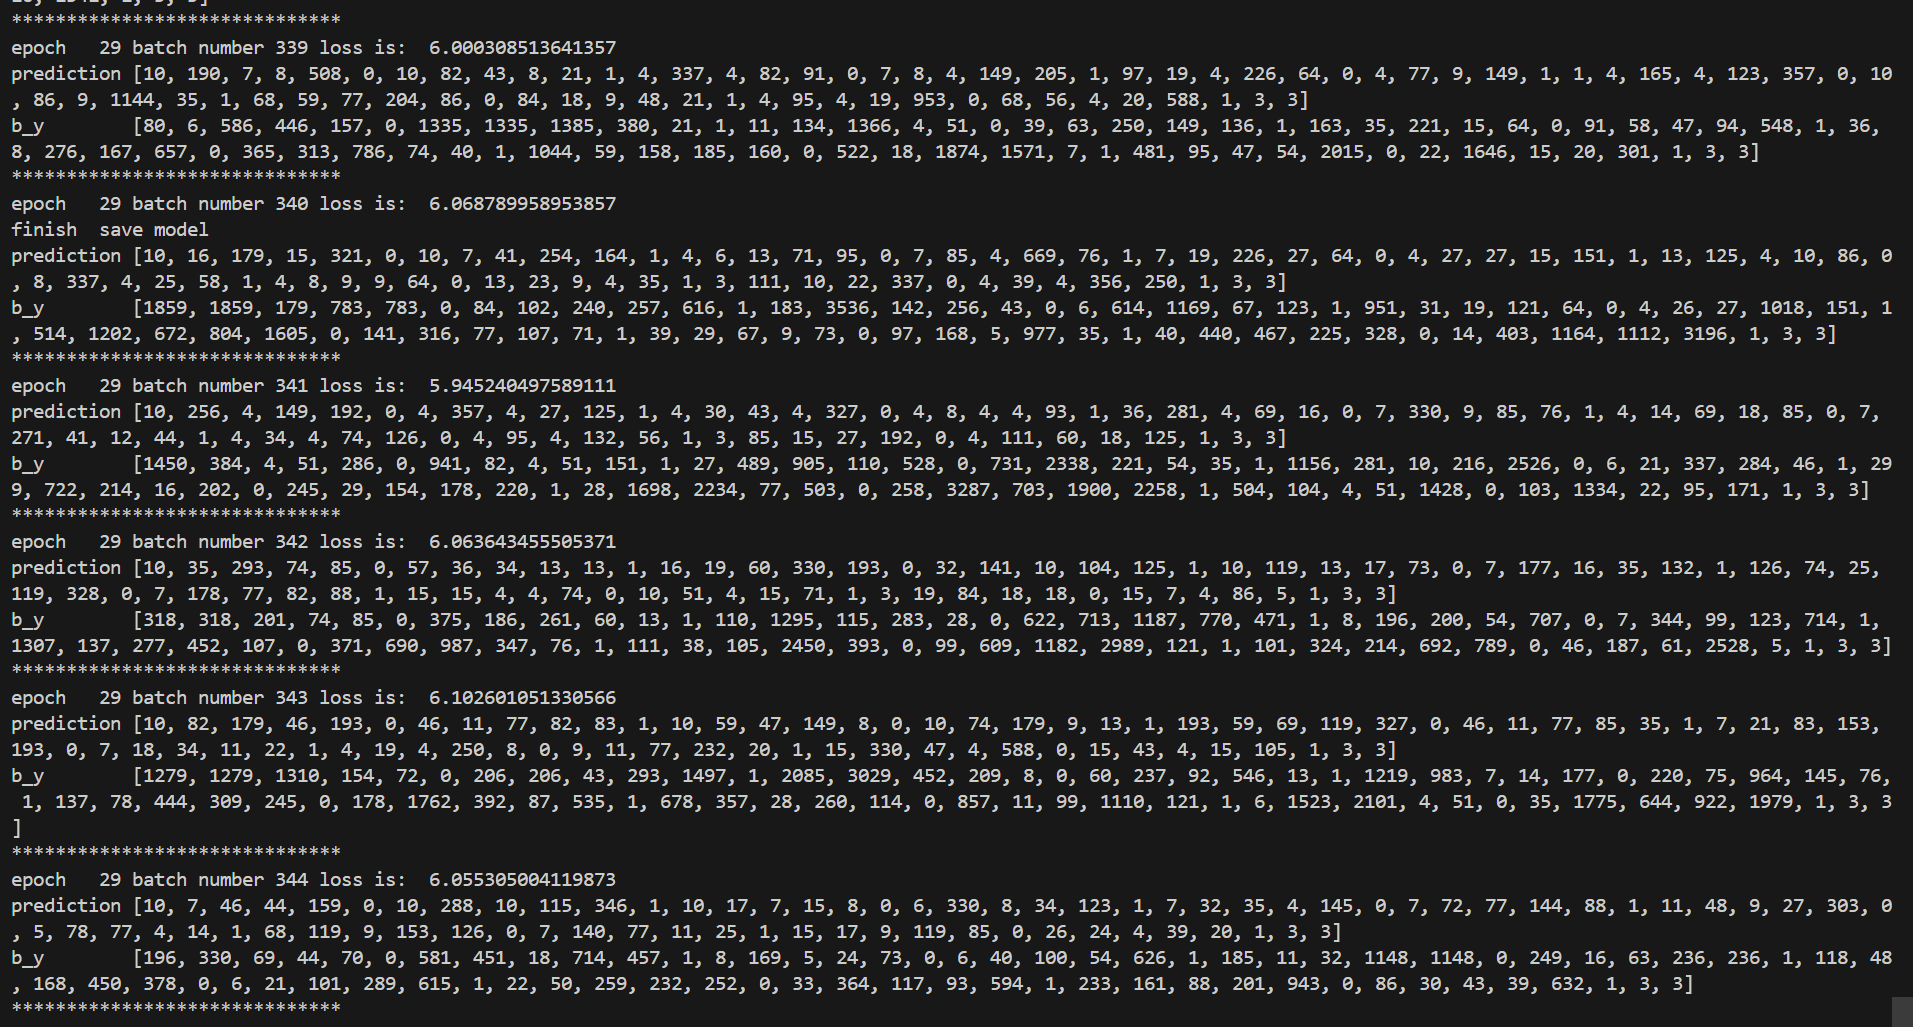
\includegraphics[width=0.85\textwidth]{training_screenshot.png}
    \caption{LSTM模型训练过程截图}
    \label{fig:training}
\end{figure}

\subsection{诗歌生成结果}

使用以下7个汉字分别作为开头字（begin word），由训练好的LSTM模型生成诗歌，结果如下：

\begin{table}[H]
\centering
\caption{以指定开头字生成的诗歌}
\label{tab:poems}
\begin{tabular}{cl}
\toprule
\textbf{开头字} & \textbf{生成诗歌} \\
\midrule
日 & 日云浮树，风光生九州。不知何处客，不见此中人。何事蓬山老，何年 \\
红 & 红玉风。上国无人知，今朝有一言。何当一何在，时复一相思 \\
山 & 山古树，风起春光满。若教无子知难，不得中生作老 \\
夜 & 夜悠悠，风起春风起，夜色不可见，一枝无处春不知何处在，不见此 \\
湖 & 胡水上天。不知何处，乐以以为。 \\
海 & 海草年尘。风光有花气，不见此心中。何事不可见，一枝无处春 \\
月 & 月，悠悠，风流不可寻。不知何处，万国在天。 \\
\bottomrule
\end{tabular}
\end{table}

\subsection{生成结果截图}

% ===== 请将生成结果的终端截图替换下方占位符 =====
\begin{figure}[H]
    \centering
    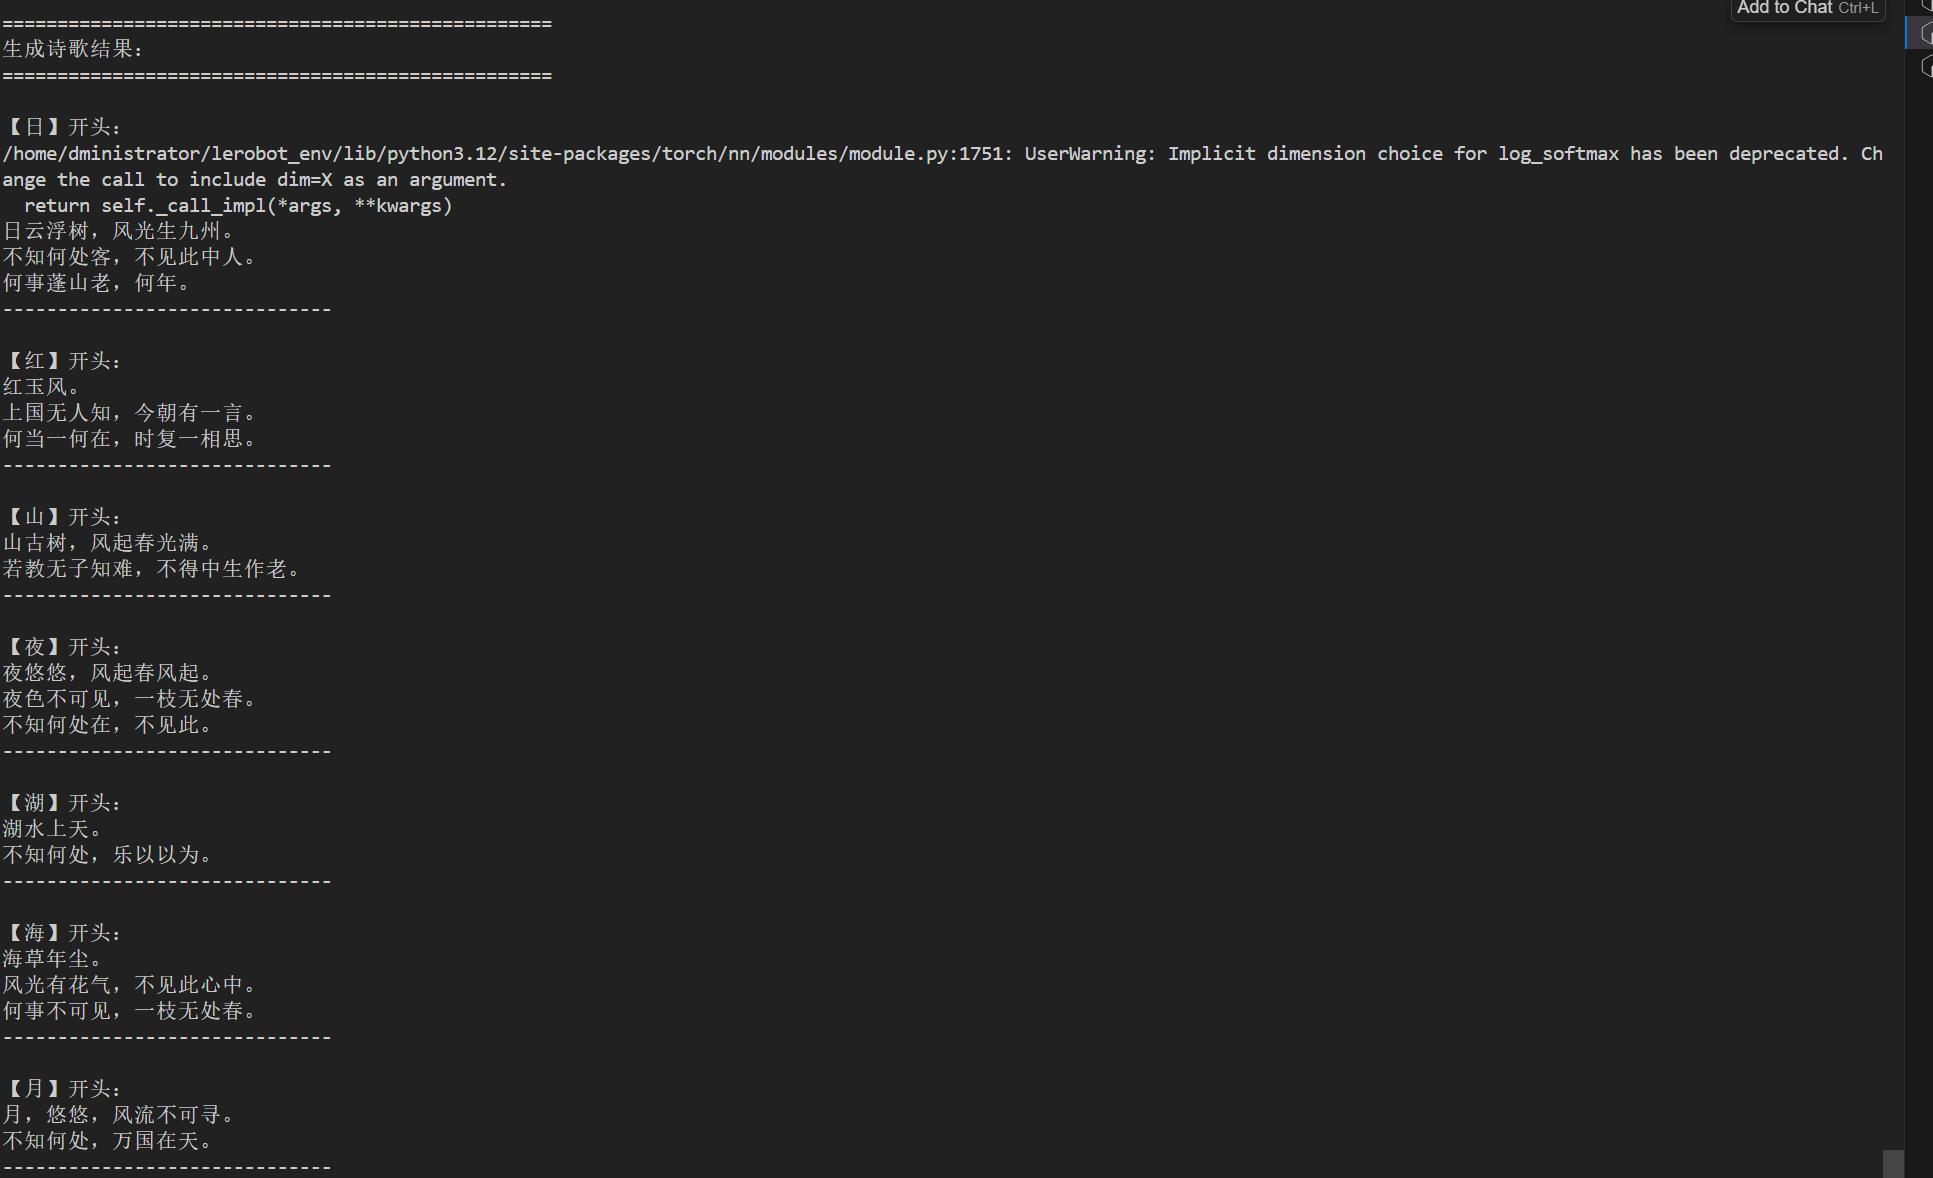
\includegraphics[width=0.85\textwidth]{generation_screenshot.png}
    \caption{诗歌生成终端运行截图}
    \label{fig:generation}
\end{figure}

%=============================================================
\section{实验总结}
%=============================================================

\subsection{实验收获}

\begin{enumerate}
    \item \textbf{深入理解了RNN系列模型}：通过本次实验，对RNN、LSTM、GRU三种循环神经网络的结构原理有了更加深入的认识。特别是LSTM通过门控机制解决长距离依赖问题的思想，在实际编码中得到了验证。

    \item \textbf{掌握了序列生成的建模方法}：理解了语言模型的本质——通过学习 $P(w_t | w_1, w_2, \ldots, w_{t-1})$ 的条件概率分布，实现逐字符的自回归生成。训练时使用Teacher Forcing策略，生成时使用贪心解码。

    \item \textbf{PyTorch实践能力提升}：通过补全LSTM的定义和前向传播代码，加深了对PyTorch中 \texttt{nn.LSTM} 接口的理解，包括隐藏状态的初始化、输入输出维度的对齐等。
\end{enumerate}

\subsection{存在的问题与改进方向}

\begin{enumerate}
    \item \textbf{生成质量}：当前模型生成的诗歌在语义连贯性和格律方面仍有不足，可以通过增大模型容量、使用更大的数据集或引入注意力机制来改善。
    \item \textbf{解码策略}：实验中使用了贪心解码（取概率最大的字），可以尝试\textbf{采样解码}（按概率分布采样）或\textbf{Beam Search}等策略，以增加生成诗歌的多样性。
    \item \textbf{格律约束}：古诗对平仄、押韵有严格要求，可以在生成过程中加入格律规则作为额外约束，提升生成诗歌的形式美感。
\end{enumerate}

%=============================================================
\section*{参考文献}
%=============================================================

\begin{enumerate}[label={[\arabic*]}]
    \item Xingxing Zhang and Mirella Lapata. 2014. Chinese poetry generation with recurrent neural networks. In \textit{Proceedings of the 2014 Conference on EMNLP}. Association for Computational Linguistics, October.
    \item Hochreiter S, Schmidhuber J. Long short-term memory[J]. \textit{Neural Computation}, 1997, 9(8): 1735-1780.
    \item Cho K, van Merrienboer B, Gulcehre C, et al. Learning phrase representations using RNN encoder-decoder for statistical machine translation[C]. \textit{EMNLP}, 2014.
\end{enumerate}

\end{document}
